\chapter{Magnetooptika}
V experimentální části práce se zabýváme měřením magnetooptických jevů. V~této kapitole shrneme základy magnetooptiky a nejdůležitější vztahy pro provedené experimenty. Hlavním zdrojem této kapitoly je diplomová práce \cite{Subrt} a v~případě kapitoly \ref{kap_VoigtMLD} o Voigtově jevu a MLD je to \cite{Tesarova}.

Magnetooptickými jevy nazýváme jevy, při kterých dochází k interakci elektromagnetického záření s magnetickou látkou. 

Nenulová magnetizace v látce může mít za důsledek její optickou anisotropii. Látka pak může mít v různých směrech rozdílný reálný index lomu nebo absorpční koeficient, případně se tyto dvě veličiny mohou lišit pro levotočivou a pravotočivou kruhovou polarizaci.

Po průchodu (případně odrazu) laserového světla takovou látkou dojde vlivem anizotropie indexu lomu nebo absorpčních koeficientů ke změně jeho polarizačního stavu. Změní se elipticita a dojde k rotaci roviny polarizace. Studiem změny polarizačního stavu lze následně dostat informaci o magnetizaci ve vzorku. Sledováním magnetizace při působení vnějšího magnetického pole je potom možné studovat magnetické vlastnosti látky, např. koercitivní pole.

V magnetooptice se rozlišují dvě základní geometrie
\begin{itemize}
	\item Voigtova geometrie: světlo se šíří kolmo na směr magnetického pole
	\item Faradayova geometrie: světlo se šíří rovnoběžně na směr magnetického pole
\end{itemize}
V této práci pracujeme pouze ve Voigtově geometrii.


Magnetooptické jevy se klasifikují následujícím způsobem. Pokud se pro dvě ortogonální polarizace liší reálný index lomu, označujeme jev jako \emph{dvojlom} (birefringence). Pokud se liší absorpční koeficienty, označujeme jev jako \emph{dichroismus}. 

Dále jevy dělíme podle jejich normálních módů, tj. jestli se daný parametr liší pro dvě lineární či dvě kruhové (circular) polarizace. Lineární jevy nastávají~ve Voigtově geometrii, zatímco kruhové ve Faradayově. 

Rozlišujeme tedy následující jevy
\begin{itemize}
	\item MCD (magnetic circular dichroism)
	\item MLD (magnetic linear dichroism)
	\item MCB (magnetic circular birefringence), také Faradayův jev
	\item MLB (magnetic linear birefringence), také Cotton-Moutonův či Voigtův jev.
\end{itemize} 

Lineární jevy jsou sudé v magnetizaci, kruhové jevy jsou liché v magnetizaci. Jevy sudé v magnetizaci se obecně měří hůře, protože není možné signál oddělit od experimentálních artefaktů jako u lichých jevů.


Mechanismus rotace roviny polarizace vlivem MLD je ilustrován na obr. \ref{mld_subrt}.

\begin{figure}[htbp]\centering
	\qq{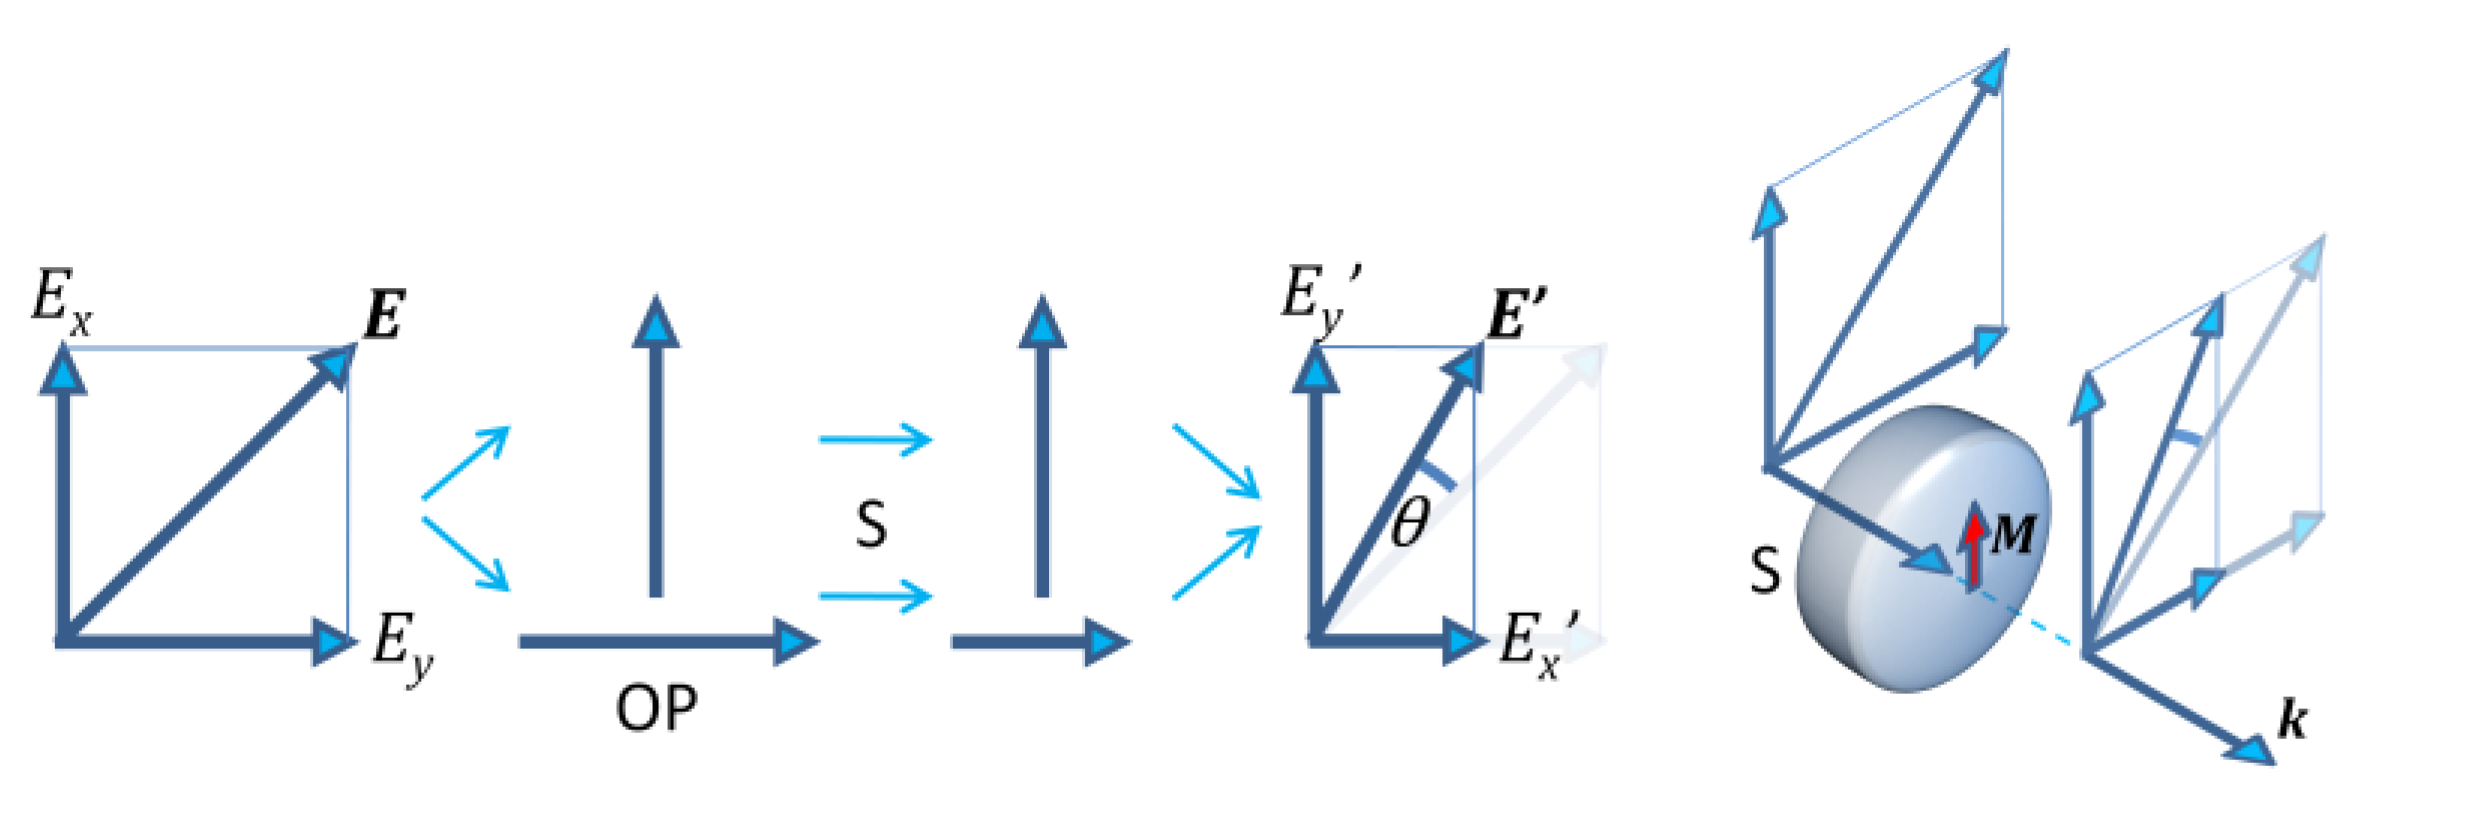
\includegraphics{Subrt_34}}
	\caption{Rotace roviny polarizace vlivem MLD \cite{Subrt}.}\label{mld_subrt}
\end{figure}

V reflexní geometrii se někdy magnetooptické jevy označují jako MOKE (magnetooptical Kerr effect), které se dále rozlišují podle vzájemné orientace vlnového vektoru, roviny vzorku a magnetizace, viz obr.~\ref{kerr_subrt}.

\begin{figure}[htbp]\centering
\qq{	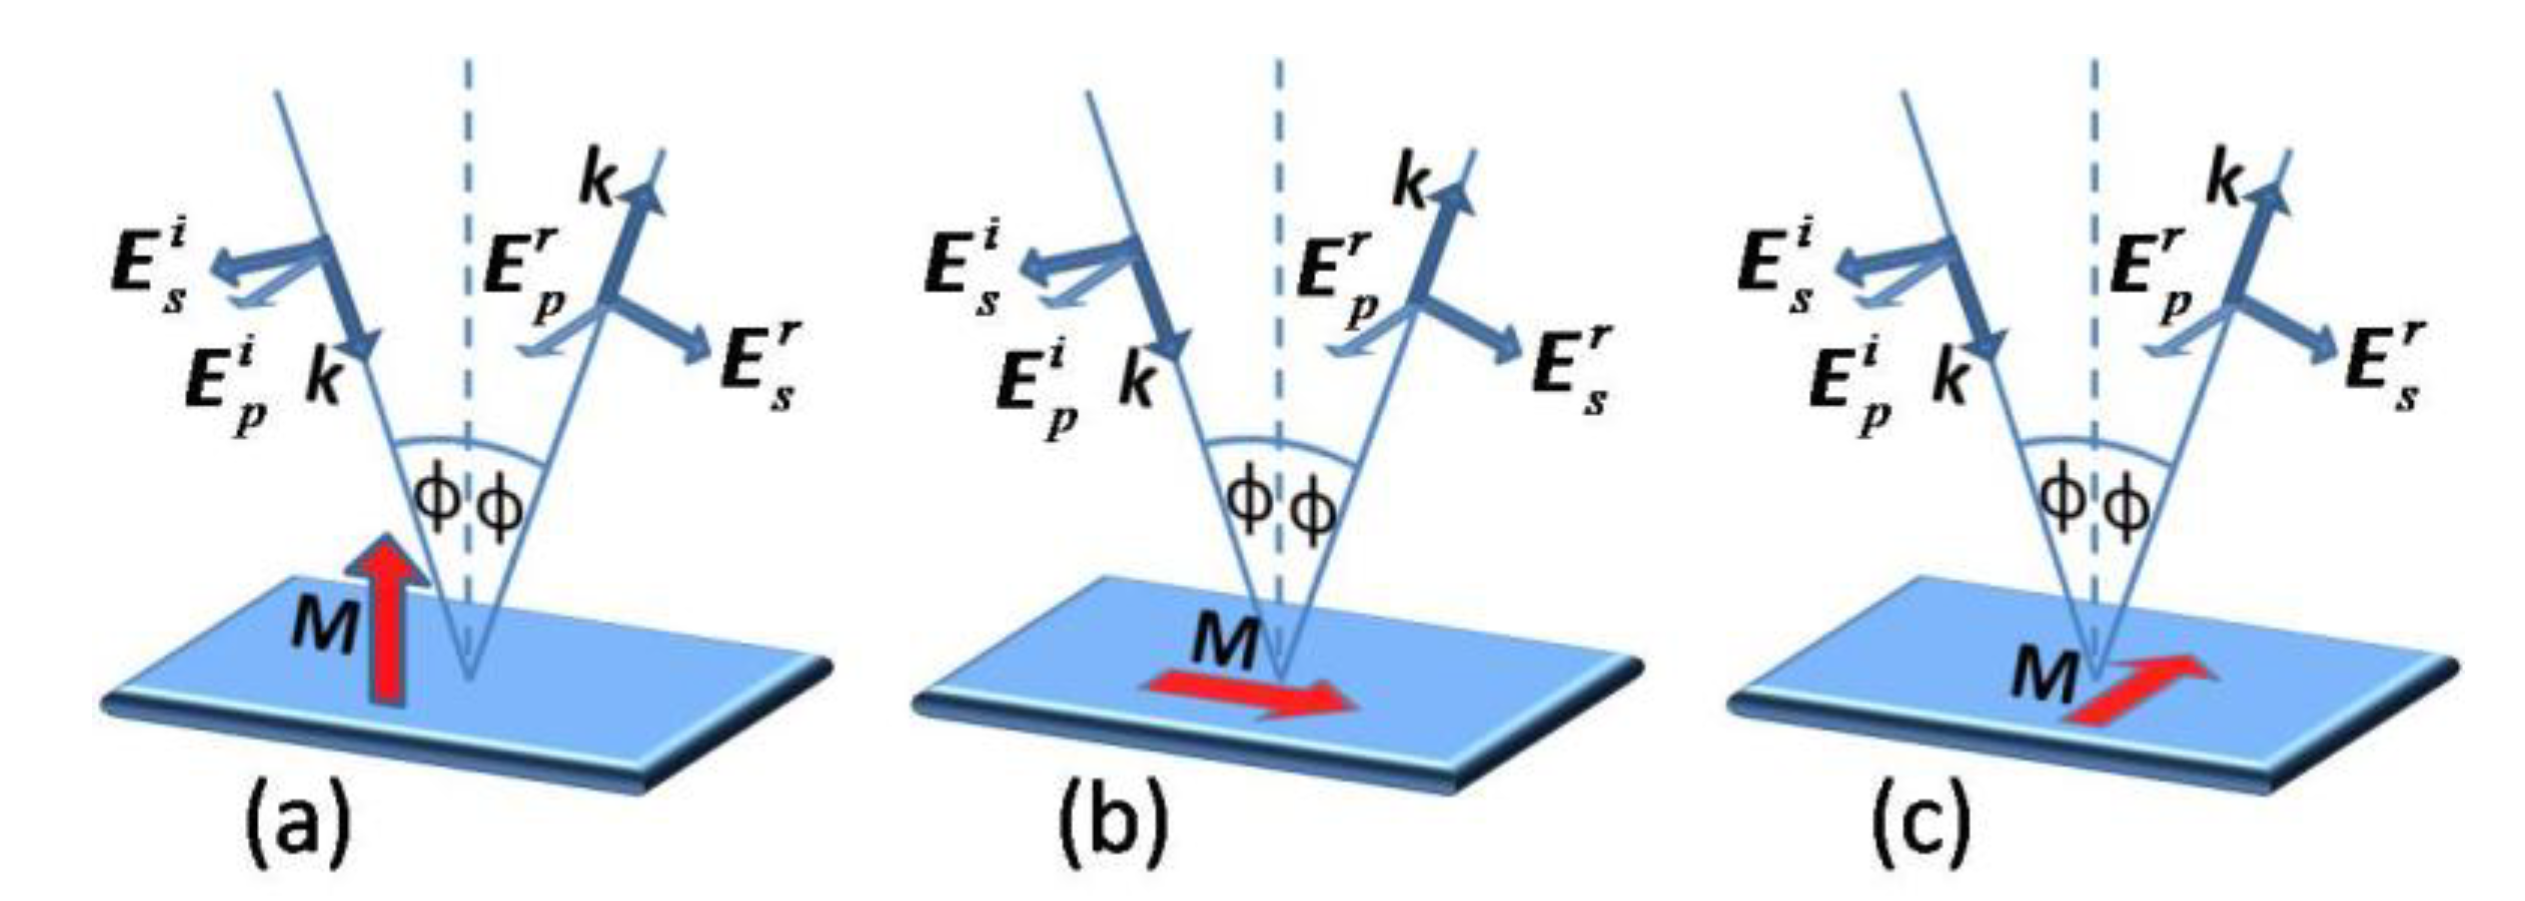
\includegraphics{Subrt_35}}
	\caption{MOKE: (a) polární, (b) longitudinální, (c) transversální \cite{Subrt}.}\label{kerr_subrt}
\end{figure}

\section{Voigtův jev a MLD v reflexní geometrii} \label{kap_VoigtMLD}

MLD je kvadratický (v magnetizaci) magnetooptický jev původně pozorovaný v transmisní geometrii jako dichroismus lineárně polarizovaného světla. Rozdílné absorpční koeficienty pro polarizaci kolmou a rovnoběžnou na směr magnetizace způsobují po průchodu stočení roviny polarizace \cite{cit1}, \cite{cit2}. 

Posléze se jako MLD začal označovat i jiný magnetooptický jev v reflexní geometrii při kolmém a téměř kolmém dopadu \cite{cit3}. Rozdílný reálný index lomu pro obě lineární polarizace způsobuje rozdílnou odrazivost, což má podobně jako u transmisního MLD za následek stočení polarizace. Jev je standardně označován jako MLD, přestože je analogický MLB.

Pro konzistenci s terminologií používanou na našem pracovišti se budeme držet následujícího názvosloví: pokud je studovaný jev rozdílná odrazivost pro lineární polarizaci v různých směrech, jedná se o MLD. Pokud je studovaný jev rotace roviny polarizace, jedná se o Voigtův jev, přestože mají oba jevy původ ve stejné fyzikální skutečnosti. V dalších kapitolách budeme měřit stejné fyzikální veličiny zároveň pomocí MLD i Voigtova jevu a získaná data z obou měření budeme označovat právě tímto způsobem.

MLD signál je v tomto kontextu definován jako \cite{Tesarova}
\begin{equation}
\mld[\si{\radian}]=\frac{1}{2}\frac{I_R^\paral - I_R^\perpen}{I_R^\paral + I_R^\perpen}=\frac{1}{2}\frac{r^2_\paral-r^2_\perpen}{r^2_\paral+r^2_\perpen} \,,
\end{equation}
kde $I_R^\paral$ resp. $I_R^\perpen$ jsou intenzity odraženého světla polarizovaného rovnoběžně resp. kolmo na magnetizaci. Podobně $r_\paral$ a $r_\perpen$ jsou koeficienty reflexe elektrické intenzity (intenzitní odrazivost je rovna $r^2$).

Pokud v rovině vzorku označíme úhel $\phM$ jako směr magnetizace a úhel $\beta$ jako rovinu polarizace\footnote{Soustava souřadná je definovaná v kapitole \ref{exp_usporadani}, vztahy v této kapitole jsou na ní však nezávislé}, pak pro stočení polarizace ($\Delta\beta=\beta^\prime-\beta$) platí \cite{Tesarova} 
\begin{equation}
\tan(\Delta \beta)=\frac{(r_\paral-r_\perpen)\tan(\phM-\beta)}{r_\paral + r_\perpen \tan^2(\phM-\beta)} \,,
\end{equation}
což je pro malé úhly ($r_\paral /r_\perpen \approx 1$)
\begin{equation} \label{rotace_polarizace}
\Delta \beta = \pmld \sin \left[ 2(\phM-\beta) \right] \,,
\end{equation}
kde $\pmld=\num{0.5}(r_\paral/r_\perpen -1)$ je MLD magnetooptický koeficient.

Přestože má situace $\Delta\beta=0$ jasný fyzikální význam (dopadající a odražená polarizace jsou totožné), jsme často schopni určit pouze průběh $\Delta\beta$ až na aditivní konstantu. Dále, zejména v kapitole s experimentálními výsledky, označuje $\Delta\beta$ odchýlení od určitého arbitrárně zvoleného směru.

V přiblížení $r_\paral /r_\perpen \approx 1$ platí
\begin{equation}
\pmld=\frac{1}{2}\frac{r^2_\paral-r^2_\perpen}{r^2_\paral+r^2_\perpen} \,.
\end{equation}

Voigtův jev je tedy polarizačně závislý podle vztahu \eqref{rotace_polarizace} a je největší, když rovina polarizace svírá s magnetizací úhel \ang{45}.

MLD pozorujeme prostřednictvím celkové odražené intenzity $I'$. V příloze \ref{odvozeni_mld} je odvozeno, že v našem přiblížení platí
\begin{equation}
I^\prime=I_0 R \left[1 + 2\pmld \cos[2(\phM-\beta)]\right] \,,
\end{equation}
kde $I_0$ je dopadající intenzita a $R$ je odrazivost vzorku.
Pro studium MLD zavedeme veličinu
\begin{equation} \label{e:Bdef}
B:=\frac{I^\prime}{I_0 R}-1 \,.
\end{equation}

Potom
\begin{equation}
B=2\pmld \cos[2(\phM-\beta)] \,.
\end{equation}
MLD je tedy největší, když porovnáváme odrazivost pro polarizace ve směru rovnoběžném a kolmém na~magnetizaci.